\section[Multichain-based certificate verification]{Multichain-based certificate management}
\begin{frame}
\frametitle{Multichain-based certificate management}
\begin{alertblock}{Multichain}
	\begin{itemize}
		\item fork of the Bitcoin source code
		\item hugely simplifies private Blockchains creation and management
		\item lot of settings available
		\item node permission control
		\item arbitrary-sized data field in transactions
		\item very well documented
	\end{itemize}
\end{alertblock}
\end{frame}

%% TODO: move this slide to the next section

\begin{frame}{Comparison}

\begin{tabular}{|c|c|c|c|}
\hline 
  & Smart contracts & OP\_RETURN & Multichain \\ 
\hline 
Usability - customization & - & - & + \\ 
\hline 
Cost & - & - & + \\ 
\hline 
Compatibility with existing PKIs & - & + & + \\ 
\hline 
Permissions & - & - & + \\ 
\hline 
Size of certificates & + & - & + \\ 
\hline 
Scalability & + & - & - \\ 
\hline 
\end{tabular} 

\end{frame}


\begin{frame}
	\frametitle{Design}
	\begin{center}
		\begin{tikzpicture}
		[node distance=1cm and 4cm]
		\node[label=above:{CA}](CA) {{\LARGE \faUser}};
		\pause
		\draw[-] (CA) to (d3);
		\node[below = of r.south] (d3) {sign};
		\node[label=below:{Cert}, below = of d3.south] (cacert) {{\Huge \faFileTextO}};				\draw[->] (d3) to (cacert);
		
		\pause
		
		\node[right=of CA.east, label=above:{secure connection}](secure){};
		\node[label=above:{Miner}, right = of secure.east](Miner){{\LARGE \faUser}};
		\draw[->] (CA) to (Miner);
		\pause
		\draw[-] (Miner) to (d4);
		\node[below = of r.south, below = of Miner.south] (d4) {produce};
		\node[label=below:{Transaction}, below = of d4.south] (trans) {{\Huge \faFileTextO}};
		\draw[->] (d4) to (trans);
		
		\end{tikzpicture}
	\end{center}
\end{frame}

\begin{frame}
	\frametitle{Scenario}
	\begin{alertblock}{}
		\begin{enumerate}
			\item final user visits a website with web browser
			\item classical identity verification is used (PKI)
			\item browser plug-in installed on the user browser
			\item local daemon is running, waiting for queries
			\item plugin-in retrieves certificates, asking to daemon if such a certificate is valid
			\item displays whether certificates should be trusted or not
		\end{enumerate}
	\end{alertblock}
\end{frame}


\begin{frame}
	\frametitle{Demo}
	\begin{center}
		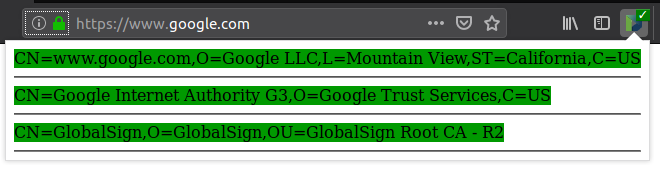
\includegraphics[scale=0.4]{figs/green_certs.png}
		
\includegraphics{figs/green_tick.png}
	\end{center}
\end{frame}

\begin{frame}
	\frametitle{Demo}
	\begin{center}
		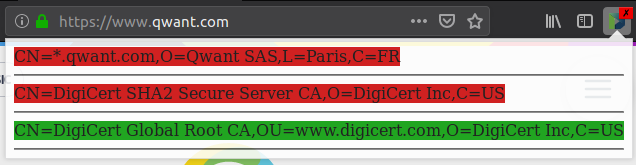
\includegraphics[scale=0.4]{figs/red_certs.png}
		
\includegraphics{figs/red_mark.png}
	\end{center}

%% TODO: move this slide to another section

\begin{frame}{Cost and scalability}

	\begin{exampleblock}{Use case: Let's Encrypt}
		\begin{itemize}
			\item Certification authority
			\item Delivered 100M certificates over 20 months
			\begin{itemize}
				\item More than 160K per day
			\end{itemize}
		\end{itemize}
	\end{exampleblock}
	
	\begin{exampleblock}{Application to multichain-based certificates management}
		\begin{itemize}
			\item Around 280 Go of memory for 100M certificates
			\item The whole blockchain has to be read when searching for a specific certificate
			\begin{itemize}
				\item Ideally, nly the delivery day would have to be checked in the blockchain
			\end{itemize}
		\end{itemize}
	\end{exampleblock}

\end{frame}